\chapter{Advanced Editing}%
\label{cha:advanced_editing}

\section{Proxy}%
\label{sec:proxy}

Working with videos that have large image geometry can greatly impede editing.  Instead you can substitute \textit{proxies} which will create smaller video image files from the original file that can then be edited more quickly.   When you are done working on this smaller scale, you will need to bring up the Proxy settings menu again, and change the Scale factor back to the Original size so that all of your edits/work take affect on that original higher quality video on the timeline.  

To use this feature, select \texttt{Settings $\rightarrow$ Proxy settings} and change the Scale factor from Original size to your downsized choice.  You can choose ffmpeg as the File Format and a choice of various codecs associated with that.  A good choice is the default of mpeg which can usually be quite fast.  In addition, to modify values for that codec, click on the wrench icon.  When you have completed your choices, just click OK, and then the video tracks will be rendered. This may take some time, but previous proxy renders will be reused.  
The proxy videos will be added to your assets in a separate Proxy folder, and the video track edits will use the proxies.
The assets in both the Media folder and Proxy folder will look proxied when dragged to the Viewer although the scale may be different.
Proxy downsizing renders all loaded tracks, but only work on the $1^{st}$ video layer of any multi-layer media.  Rendered proxy media is saved in the same directory as the original media.
However, if you proxy your session, the clips do not get proxied to the Proxy folder, but if you Drag and Drop the clip from the Clip folder to the Viewer or the Timeline, you will see that it too is proxied.  
As usual, you can delete proxy files from the project or disk in the Resources window if you no longer want to retain them.
And you can save your project either as proxied or not.

Because Proxy works on the original media in all circumstances, when you resize the
media in the Resources window, it does not actually resize the media but puts it in
a "buffer" in that format. This might lead to some confusion for the user who
expects this resizing to be maintained when disabling Proxy for that media. However,
that does not happen because the resize is only in a buffer and not in the original
media. This result is different than in the case of media "edits", like cuts or
adding plugins because this information is not in a buffer but rather part of the
copy "Editing Decision List" (EDL).

You can also nest clips while in a proxied state, but you can not drag the proxied nested clips
to the viewer or the timeline.
If you create proxies for Nested clips they will be saved in \texttt{\$HOME/Videos} unless you modify that in
\texttt{Settings $\rightarrow$ Preferences, Interface} tab, \textit{Nested Proxy Path}. 

There are two ways that the proxy files can be used, with or without input scaling. When the proxy is done without rescaling, the Mask, Camera and Projector automations are re-scaled accordingly. In this situation, the entire project will be re-sized so that the session is in the resized geometry.  Not all plugins are useful when the project is rescaled, because the keyframe data must be in the original geometry.  In this case, you can use the rescaler, by enabling \textit{Use scaler (FFMPEG only)}. This has the added advantage that the project size does not change and the proxy media is down-scaled as usual and up-scaled on read-in, which means the project editing is done in full scale.   Since decoding is done on smaller video, there is a time savings, but all rendering is done full scale.  The main reason for using \textit{scaler} is that it does not change the image coordinate data, so that automation and plugin parameters will be in the original project geometry.   This is not as fast as the first option, but is a performance gain, and may be needed if you are using plugins that need coordinate data such as the Title plugin.  As noted, the scaler only works on ffmpeg video formats.

In the upper right hand corner of the main window, there is a toggle button to easily switch back and forth when you have a proxied file on the timeline.  The icon is to the left of the FF icon.  It will have the letter “P” as the icon for Proxy or if \textit{Using Scaler}, the letter “S”. \quad 
\includegraphics[height=\baselineskip]{proxy-01.png} \quad This quick switch is especially useful when editing and you need to see a better image temporarily.

\begin{figure}[htpb]
	\centering
	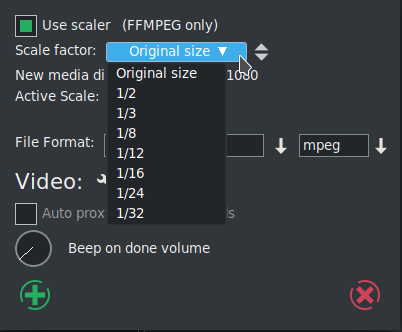
\includegraphics[width=0.5\linewidth]{proxy-02.png}
	\caption{Proxy settings dialog}
	\label{fig:proxy-02}
\end{figure}

Screencast in figure~\ref{fig:proxy-02} shows the Use scaler checked so you can still use plugins and the original project size is kept.  The Scale factor pull-down gives you available size options.  Note the new media dimensions shown (partially covered).  If the size is an odd number, 1 is added to make the dimensions both even numbers.

In the case of the scaler checkbox, it will retain that setting for ease of use.

There is also a convenient \textit{Beep on done volume} dial included so that you can work on other tasks until there is an audible notify of completion.  The default volume is set to 0 for no audible notify.

A good choice for proxy settings with 1080p source video is:

\begin{lstlisting}[numbers=none]
Scale Factor: 	1/4
Use Scaler:	unchecked
File Format:	FFMPEG - mpeg
Video Preset:
Compression:	mpeg.mpeg
Bitrate:	1800000
Quality:	-1
Pixels:		yuv420p
\end{lstlisting}

If you get errors for some videos, such as those with strange variable bit rate or some types of files made on a smartphone, a usually reliable alternative is to change the following parameters:

\begin{lstlisting}[numbers=none]
File Format:	FFMPEG - mov
Video Preset:
Compression:	mov.mov
\end{lstlisting}

Or if you want small files with high image quality, a File Format of m2ts is optimal.  For example a 1 GB file can be reduced to 50 MB with scale $\frac{1}{2}$. 

Checking the \textit{Auto proxy/scale media loads} results in any additional media loads to be automatically proxy scaled.  However, single frame media such as PNG or JPEG \textit{stills}, can not be scaled to \textit{stream} media.  If this type of media exists, you should \textit{use scaler}.

If you get error messages when creating proxies, check the Video wrench settings.  These usually default to values that are expected to work correctly for the \textit{File Format} and codec you selected but they can be changed and may result in errors.  If you get an error message of \textit{check\_frame\_rate failed} followed by \textit{Error making proxy} in the popup Errors window, do just that and check the Frame rate value by going to the Resources window, Media folder, and use the right mouse button for the Info option for that specific media in question.  You can change the frame rate in this window to a more codec acceptable value.  Different codecs may have different legal values.

More specific information on which plugins need to use scaler is provided here next.  If the keyframe data uses coordinate data that is absolute, then the scaler should be used.  If the data is normalized (like always $0-100\%$) then the proxy can be done without the scaler.  The session geometry format, shown in \texttt{Settings $\rightarrow$ Format} as $width \times height$, is changed if the scaler is not used to cause all of the data to be in the reduced format.  If this affects the plugin operation, then scaler should be used.  Examples of plugins that need the scaler are: Title, AutoScale, Scale, ScaleRatio, and Translate.  Most others are safe to use without scaling.

\section{Transcode}%
\label{sec:transcode}

Transcode, an option under the \textit{Settings} pulldown right next to the Proxy settings option, is a type of full resolution \textbf{1:1 Proxy}.
The process of transcoding works directly from the resource; it is independent of the timeline. 
All of the loaded asset media will be converted, that is, rendered in the selected format and loaded onto the timeline. 
Menu choices besides the usual File Format and File Type include: \textit{Tag suffix} (to add to media filename), \textit{Remove originals from project}, \textit{Into Nested Proxy directory} (an option to have the file saved here instead of the location of the original media), and \textit{Beep on done} volume.

The settings of the project have an effect, for example the dimensions are taken into account. The resulting files are also larger than if they were created directly with ffmpeg.
Transcode works for videos with or without audio and even single frame files, like png's.
If you have a video file that also contains audio, and you convert only the video, the original audio will stay on the timeline if do not check \textit{Remove originals from project}. Or vice versa if audio converted and not video.
Multiple stream media will only transcode the first stream (this would be like the TV channel recordings in the United States).
You will get an error message if you already have a transcoded file in the selected format with the same suffix name and try to transcode it again with a different selection made -- you will have to delete that file first. An example would be
an already converted file that has both video and audio and now you request video only. 

The BIGGEST gain from using this is if you have media that is not \textit{seekable}, that is, you can play it from the beginning but can not move to another spot and have the audio or video play correctly. A video file with no keyframes makes seeking next to impossible, but then a Transcode generally adds these keyframes. 


\section{OpenEDL}%
\label{sec:openedl}

To edit EDL that is included with your project as Clips, Nested
Clips, Referenced File, or Xml you can use the option \textit{Open
	EDL} in the Resources window for the highlighted media.  Then with
a simple button click you can return to your main timeline project.
For example, if you have a nested clip that originally had several
plugins added to it before it was nested, you can edit those plugin
parameter values. Previously to make any changes to these types of
EDL you had to remake the whole clip from scratch.

Here is how this works. In the Clip or Media folder or on a timeline
EDL edit, the option \textit{Open EDL} for the highlighted clip or
nested clip is available so that when you choose this option, that
EDL will be brought up on the timeline superseding the current EDL
that exists on the timeline.  Now, once the clip is open on the
timeline, you can edit it however you want. The previous timeline
EDL is \textit{pushed onto a stack} so it can be recalled by
\textit{popping the stack} with a click of the left mouse button in
the upper right hand corner of the timeline to the left of the
\textit{shell cmds} icon.  Initially this button displays a 0 to
indicate your initial timeline/project.  Then this button will read
1 if you choose \textit{Open EDL} and then back to 0 and your
original timeline with the left mouse click.  You can go several
levels deep so instead of 1, it could be 2, 3, $\dots$ but this
requires some thought to avoid potential confusion.

An example of a typical set of steps to follow is:
\begin{enumerate}
	\item Load your media using insertion strategy of \textit{Replace
		current project}.  There will be number 0 in the upper right hand corner
	of the main menu with the tooltip of \textit{Close EDL}.
	\item Highlight a selection on the timeline and press the
	\textit{To clip} icon and click the green checkmark OK.
	\item In the Resources window, open the Clip folder and you will
	see that Clip 1 is present.
	\item Highlight Clip1 and right mouse the item to bring up
	available options and select \textit{Open EDL}.
	\item Now you will see the timeline change from the original
	media to just the clip content and the number in the upper right hand
	corner will change from 0 to 1.
	\item Add a visible effect, like AgingTV to the timeline.
	\item Click on the number 1 in the main menu bar to see the timeline
	restored to the original media.
	\item Drag the clip from the Resources Clip folder to the
	timeline and you will see the AgingTV effect.
\end{enumerate}

You can follow the same steps as above by first using the option
\textit{Nest to media} in the Clip folder which nests the clip and
moves it out of the Clip folder to the Media folder.  Then use
\textit{Open EDL} on the Nested EDL in the media folder.  When you
Open EDL and edit the changes, those changes will take affect on any
and all occurrences of that nested clip on the current and/or
original timeline. The option to unnest that clip and put that back
into the Clip folder is the option \textit{EDL to clip}.  The nested
clip is still in the Media folder.  It will now have a name of the
next available Clip number but the comment contains the previous name so
you can tell where it came from.

Instead of using the number on the main menu to close the current
EDL, both the Media and Clip folders have \textit{Close EDL} options
with the left mouse button. Clicking on the number button is quick and
easy but for infrequent usage it is not obvious, whereas if you use
\textit{Open EDL} you see \textit{Close EDL} right below that and so
it is very obvious.  In addition in the case of where you have
opened a EDL, and you no longer see that clip in the folder, the
right mouse button where no media is highlighted will also display
the Close EDL option.

%\pagebreak
\begin{figure}[h]
	\centering
	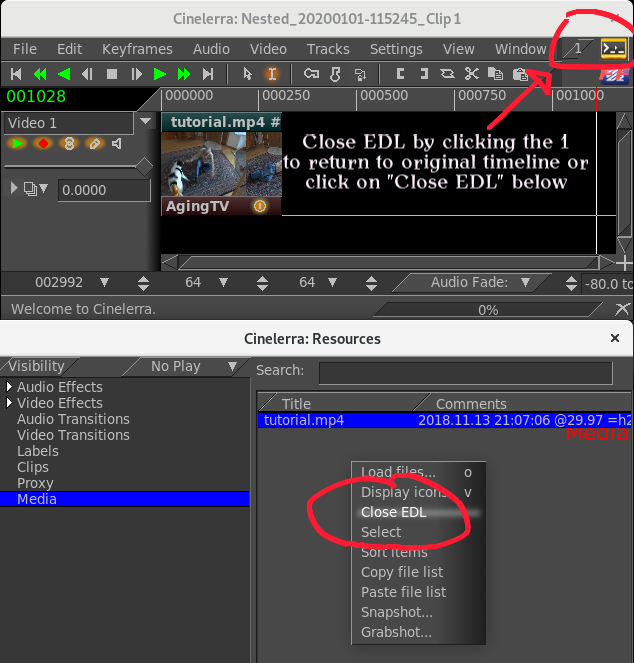
\includegraphics[width=1\linewidth]{editing-img001.png}
	\caption{Once you have an Open EDL, the easiest way to close it.}
	\label{fig:open_edl}
\end{figure}
\relax

In addition to the \textit{Open EDL} option in the Resources menu,
this option is available on the timeline when the cursor is on an
EDL-type edit. To get to this option, click on the middle mouse
button on that edit.  If it is not EDL, the option will not be
shown.  In summary:

\begin{center}
	\begin{tabular}{ll}
		\toprule
		Media folder of Resources window & Open EDL for Nested or Referenced EDLs\\
		Clip folder of Resources window & Open EDL for clips\\
		Track timeline & Open EDL for Nested or Referenced EDLs\\
		\bottomrule
	\end{tabular}
\end{center}

An aside -- when nesting and unnesting clips to take advantage of
this feature, names of the media can lead to some confusion.  For
example, if you nest a clip, the new name in the Media folder is the
word \textit{Nested} followed by an underscore with the date and
timestamp, another underscore, and then the clip name.  Then when
you unnest this Media folder clip via the \textit{EDL to clip}
option, the name will be changed in the Clip folder to the next
available Clip number.  However the comment field will reflect the
nested clip name from which it was derived.  To avoid confusion you
can easily change the name for these clips in either the Clip or
Media folder because they are not real files at this point. To do
so, highlight the clip name in Resources, click on Info and type in
a new name.

For additional safety, the \textit{Open EDL} feature includes
additional backup capabilities. Automatically \CGG{} saves a backup
when certain changes are made or you can always use the shortcut `b'
to do one yourself, although keep in mind it will be overwritten
whenever \CGG{} wants to do another backup.  Now there is a shortcut
for the backup shortcut `b' so you can keep your hand on the mouse
instead of the keyboard.  Just click on the number button in the upper right
hand corner of the main window.  If number is at 0, it backs up to
backup.xml, if at 1, it backs up to \texttt{backup1.xml} and so on
\dots up to \texttt{backup9.xml}.

When \textit{Open EDL} is invoked, the current EDL and current undo
stack are both \textit{pushed}, and the active session EDL is
replaced with the target clip/nested edl.  A new undo stack is
created, and the active \texttt{backup.xml} file name is decorated
with the stack level.  So, \texttt{backup.xml} is
\texttt{backup1.xml} when your edits are at stack level 1,
\texttt{back\-up2\-.xml} at stack level 2, and so on.  This means
that if you \textit{load backup} at stack level 1, the session will
reload from history at stack level 1, not the main session.

See a real-world workflow at appendix \nameref{sec:workflow_openedl_nested_clips}

\section{File by Reference}%
\label{sec:file_by_reference}

It is sometimes handy to have EDL assets not as a copy, but as a
reference that is automatically updated into your project.  Suppose
you have several short videos that at the end have the same credits
which include the current year such as 2019.  But now it is 2020 and
all of the videos would have to be individually updated with the new
date.  By including a \textit{Referenced File} as the EDL file type
when you create each of the videos, you can just change the one
credits xml file and the next time you load one of the videos and
render it, it will now automatically have the updated information.

The purpose of this feature is to be able to rework a smaller
section of a global master project at any time, which can be done by
an "assistant" (i.e. external software like GIMP or Inkscape, $\dots$) and then this work is automatically reflected in the
global master project.  It is for \textbf{advanced usage only}.

Up until the addition of this feature, \CGG{} has always used copies
and no direct reference in order to ensure original data is never
compromised.  In the usual case, subprojects as xmls are copied into
a master project where subprojects had been inserted, so that if you
change something in a subproject or delete a subproject, it would
have no affect on the master project.  But now with \textit{File by
	Reference}, any project that uses a referenced file will
automatically include any changes made to the referenced file when
loaded.  At the same time, if you use the EDL file NOT as a
referenced file in a project since it is then just a copy, it will
not be updated.  Because of this difference, the user needs to be
very aware of what using this feature could do.

\textbf{Use with extreme caution}.  However, there are several
built-in safety features and a warning that should never be turned
off even though it gives you the option to do so.  These include:

\begin{enumerate}
	\item When the \texttt{File, Load files} menu is opened, the EDL
	strategy will always be set to just EDL as default.  Although, if
	you use Apply and leave the Load Menu open, it will stay changed to
	what you selected until it is re-opened.
	\item When an EDL is opened as \textit{Reference}, the color of
	that file name in the Resources Media folder is different in order
	to serve as a reminder that it is special.
	\item A warning message is displayed in a popup window when you
	load a \textit{File by Reference} that reads \texttt{Other projects can
	change this project and this can become a broken link}.  Although
	you can check the warning box to never see this warning again, you
	would be well advised to not do so.  It is a great reminder of
	consequences and you will not want to be cavalier about the warning.
	Instead just use the X to dismiss the warning.
\end{enumerate}

Here is a step by step example of how you can use \textit{File by
	Reference}:
\begin{enumerate}
	\item Start up \CGG{} and use the Title plugin to create a new
	credits file.  Save as credits.xml.
	\item Start a New project and then load an existing master
	project to the timeline.
	\item Load the credits file you created in step 1 with a Load
	Strategy of Create Resources Only and with EDL Strategy as
	\textit{Reference}.
	\item Note the color change in the credits.xml filename and the
	reference comment in the Resources Media folder.
	\item Drag the credits file to an empty spot on the timeline.
	Save this new master project and quit.
	\item Start \CGG{} up again.  Load credits.xml and make a change
	to the Title and save again.
	\item Exit \CGG{}; restart \CGG{}; load your master project and
	now you will automatically see on the timeline the changes you just
	made in the previous step.
\end{enumerate}

\section{Trimming}%
\label{sec:trimming}

With some edits on the timeline it is possible to do trimming. By
trimming you shrink or grow the edit boundaries by dragging them. In
drag and drop mode or cut and paste mode, move the cursor over an
edit boundary until it changes shape. The drag handle shows as a
left or right facing fat arrow when you cursor near the clip start
or end.  If the cursor faces left, the dragging operation affects
the beginning of the edit. If the cursor faces right, the dragging
operation affects the end of the edit.

The effect of each drag operation not only depends on the behavior
button but whether the beginning or end of the edit is being
dragged. When you release the mouse button, the trimming operation
is performed.

For all file formats, other than still images, the extent of the
trimming operation is limited to the source file length. Attempting
to drag the start of the edit beyond the start of the source, limits
it to the source start. In all trimming operations, all edits which
start on the same position as the cursor when the drag operation
begins are affected. You have to disarm tracks in order to prevent
edits from being affected.

You have 6 different choices of which mouse button to use for
specific types of editing while using the drag handle.  You change
the drag handle mouse effects by using the \texttt{Settings
	$\rightarrow$ Preferences  $\rightarrow$ Interface} tab and
modifying the Editing section as shown in the next
figure~\ref{fig:trim}. The drag handle affects not only the clip you
are working on but also frequently the entire duration of all clips
on the timeline.

\begin{figure}[htpb]
	\centering
	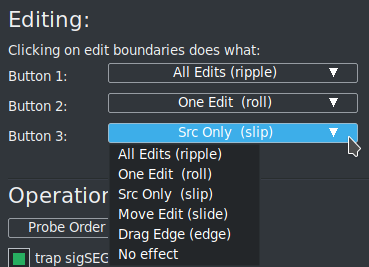
\includegraphics[width=0.5\linewidth]{trim.png}
	\caption{Default choices for mouse: Ripple for button 1; Roll
		for button 2; Slip for button 3}
	\label{fig:trim}
\end{figure}

A description of the fundamental/common terminology for choices
follows.

\begin{description}
	\item[All Edits (ripple)] shorten or lengthen the start or end
	of a single piece of media while moving all media to the right of
	that clip up or down on the timeline correspondingly.  Timeline
	duration is modified.  In a drag \textit{All Edits} operation, the
	beginning of the edit either cuts data from the edit if you move it
	forward or pastes new data from before the edit if you move it
	backward. The end of the edit pastes data into the edit if you move
	it forward or cuts data from the end of the edit if you move it
	backward. All the following edits shift. If you drag the end of the
	edit past the start of the edit, the edit is deleted.
	\item[One Edit (roll)] move the in and out point of a single
	clip without changing the timeline duration. In a drag \textit{One
		Edit} operation, nothing is cut or pasted. If you move the beginning
	or end of the edit forward, the source reference in the edit shifts
	forward. If you move the beginning or end of the edit backward, the
	source reference shifts backward. The edit remains in the same spot
	in the timeline but the source shifts.
	\item[Src Only (slip)] move the in and out point of a single
	clip without changing the timeline duration. In a drag \textit{Src
		Only} operation, nothing is cut or pasted. If you move the beginning
	or end of the edit forward, the source reference in the edit shifts
	forward. If you move the beginning or end of the edit backward, the
	source reference shifts backward. The edit remains in the same spot
	in the timeline but the source shifts.
	\item[Slide] a single clip is moved but retains its current in
	and out point; however the out point of the clip to the left changes
	and the in point of the clip to the right also changes.  Timeline
	duration remains the same.
	\item[Edge Left/Right] moves the edge of the clips.
	\item[No effect] no changes are made.  You might want to use
	this choice to prevent accidental movements.
\end{description}

The next table displays the options and results
with the Key Table here first.

\begin{lstlisting}[style=sh]
s = src media start
p = proj position
l = length
c = cut distance
rest == p+=c: for rest of clips
01 = flags edits_moved, rest_moved
\end{lstlisting}

\renewcommand{\arraystretch}{1.15}
\begin{center}
	%\caption{}
	%\label{tab:}
	% Tell table to adjust font to fix on the page using \resize	
		\begin{longtable}{lllll}
			\toprule
			&  & \textbf{Drag Left} & \textbf{Drag Right} &\\
			\midrule
			\multicolumn{2}{l}{\textit{curr s += c, l -= c; + rest}} & $\leftarrow$ & $\rightarrow$ & \textit{rest}\\
			abc12345xyz & \textbf{Ripple} left edge 11 $\rightarrow$ & abc012345xyz & abc2345xyz &\\
			\midrule
			\multicolumn{2}{l}{\textit{curr l += c; + rest}} & $\leftarrow$ & $\rightarrow$ & \textit{rest}\\
			abc12345xyz & \textbf{Ripple} right edge 01 $\rightarrow$ & abc1234xyz & abc123456xyz &\\
			\midrule
			\multicolumn{2}{l}{\textit{prev l += c; curr ps+= c, l -= c}} & $\leftarrow$ & $\rightarrow$ &\\
			abc12345xyz & \textbf{Roll} left edge 00 $\rightarrow$ & ab012345xyz & abcd2345xyz &\\
			\midrule
			\multicolumn{2}{l}{\textit{curr l += c; next ps+= c, l -= c}} & $\leftarrow$ & $\rightarrow$ &\\
			abc12345xyz & \textbf{Roll} right edge 00 $\rightarrow$ & abc1234wxyz & abc123456yz &\\
			\midrule
			\multicolumn{2}{l}{\textit{s -= c}} & $\leftarrow$ & $\rightarrow$ &\\
			abc12345xyz & \textbf{Slip} left edge 10 $\rightarrow$ & abc23456xyz & abc01234xyz &\\
			\midrule
			\multicolumn{2}{l}{\textit{s -= c}} & $\leftarrow$ & $\rightarrow$ &\\
			abc12345xyz & \textbf{Slip} right edge 10 $\rightarrow$ & abc23456xyz & abc01234xyz &\\
			\midrule
			\multicolumn{2}{l}{\textit{prev l += c; curr p+= c; next ps += c, l -= c}} & $\leftarrow$ & $\rightarrow$ &\\
			abc12345xyz & \textbf{Slide} left edge 10 $\rightarrow$ & ab012345wxyz & abcd12345yz &\\
			\midrule
			\multicolumn{2}{l}{\textit{prev l += c; curr p+= c; next ps += c, l -= c}} & $\leftarrow$ & $\rightarrow$ &\\
			abc12345xyz & \textbf{Slide} right edge 10 $\rightarrow$ & ab12345wxyz & abcd12345yz &\\
			\midrule
			\multicolumn{2}{l}{\textit{curr s -+= c, l += c; + rest}} & $\leftarrow$ & $\rightarrow$ & \textit{rest}\\
			abc12345xyz & \textbf{Edge} left edge 11 $\rightarrow$ & abc2345xyz & abc0123456xyz &\\
			\midrule
			\multicolumn{2}{l}{\textit{curr l -+= c; + rest}} & $\leftarrow$ & $\rightarrow$ & \textit{rest}\\
			abc12345xyz & \textbf{Edge} right edge 01 $\rightarrow$ & abc1234xyz & abc123456xyz &\\
			\bottomrule
		\end{longtable}
\end{center}
\renewcommand{\arraystretch}{1}

Next, a more immediate and colorful view shows these trimming
options (figure~\ref{fig:trim-color}).

\begin{figure}[htpb]
	\centering
	\includegraphics[width=0.8\linewidth]{trim-color.png}
	\caption{The 5 types of Trim: note the different lengths of the results.}
	\label{fig:trim-color}
\end{figure}

\paragraph{How to do a J-cut or L-cut} A J-cut is a split edit film
editing technique in which the audio from a following scene overlaps
the picture from the preceding scene, so that the audio portion of
the later scene starts playing before its picture as a lead-in to
the visual cut.  An L-cut is a different split edit film editing
technique in which the audio from preceding scene overlaps the
picture from the following scene, so that the audio cuts after the
picture, and continues playing over the beginning of the next scene
(figure~\ref{fig:j-cut}). To do either a J-cut or an L-cut, you
first shorten the first or second video a little.  Then you block
the audio tracks from changing by disarming the appropriate tracks.
Finally use \textit{One Edit (roll)} the cutting edge off the
videos.  Moving to the right creates a J-cut and moving to the left
creates an L-cut.

\begin{figure}[htpb]
	\centering
	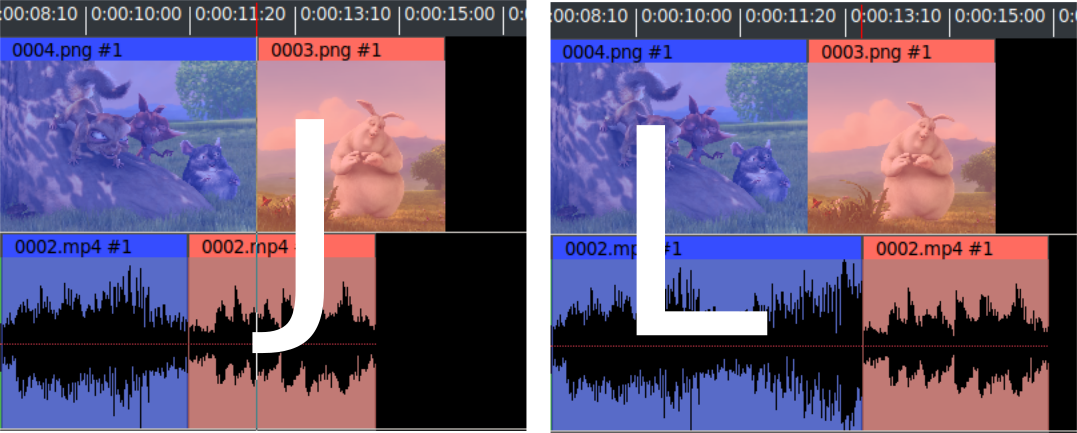
\includegraphics[width=0.8\linewidth]{j-cut.png}
	\caption{J-cut to left and L-cut to right}
	\label{fig:j-cut}
\end{figure}


\subsection{Split View in Compositor Using the Drag Handle with Trim}%
\label{sub:split_view_compositor_using_drag_trim}

The Trim Feature using the drag handle provides some good ways to
view your video while editing.  The playback position in the
compositor is updated live and the view in the compositor can be
split so that in the left half of the compositor you can see the
last frame of the left clip and in the right half the first frame of
the right clip.  Dragging edits can not be extended past the
beginning or the end.

First familiarize yourself with button operation; check your setup
by executing the following step.  In the \texttt{Settings
	$\rightarrow$ Preferences $\rightarrow$ Interface} tab, Editing
section, clicking on the edit boundaries can be set for Button 1, 2,
3 as one of the following:

\textit{Ripple}; \textit{Roll}; \textit{Slip}; \textit{Slide};
\textit{Edge} or \textit{No effect}

Now to use this feature, create a track with edits that have trims
on the left and/or the right. The edit boundary can be modified
using \textit{drag handles} at the boundary between the edits
(figure~\ref{fig:trim-display}).

\begin{figure}[htpb]
	\centering
	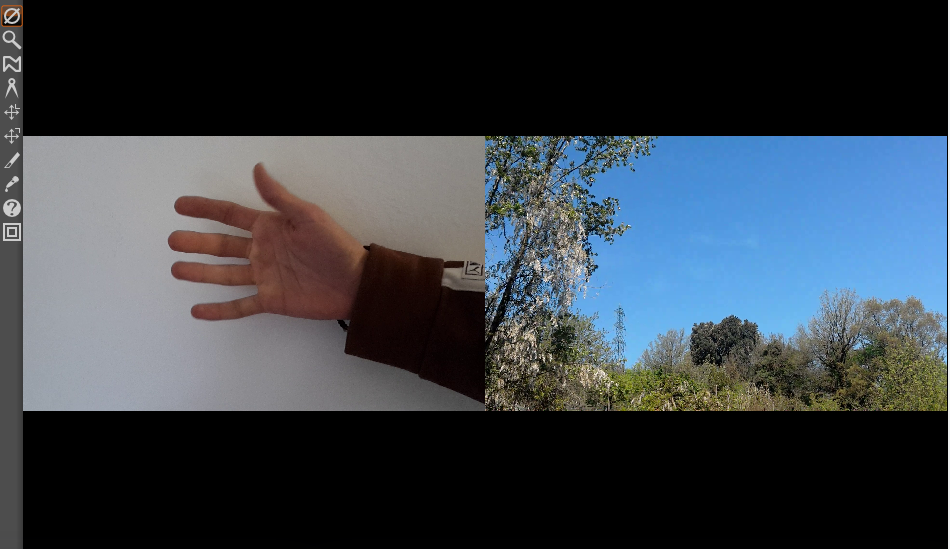
\includegraphics[width=1\linewidth]{trim-display.png}
	\caption{Split compositor screen showing the result of the Trim feature}
	\label{fig:trim-display}
\end{figure}

\begin{description}
	\item[Left Mouse Button (LMB) usage:] If you grab the edit
	handle from the right side, you will see a left arrow and dragging
	the boundary will modify the right edit playback starting time. If
	you grab the edit handle from the left side, you will see a right
	arrow and dragging the boundary will modify the left edit playback
	ending time. In both cases, the composer will show the edit endpoint
	of the changed edit.
	\item[Shift LMB usage:] The effect on the edits is the same as
	described above, but the composer will show a split screen of the
	left and right edits as they appear at the drag handle
	boundary. Dragging will only change one of the two images, since
	only one edit is being changed.
	\item[Middle Mouse Button (MMB) usage:] Both the left and the
	right edit ending/starting times are updated.  The image shown in
	the compositor will be drawn from the side of the drag grab, that is
	the left if it is grabbed from the left, and the right if it is
	grabbed from the right.
	\item[Shift MMB usage:] The effect on the edits is the same as
	described above, but the composer will show a split screen of the
	left and right edits as they appear at the drag handle boundary.
	Dragging will change both of the two images, since both edits are
	being changed.
	\item[Right Mouse Button (RMB) usage:] The start/end point of
	the current edit is moved, but the edit length is unchanged only one
	image changes since only one edit endpoint is view is updated.
	\item[Shift RMB usage:] The effect on the edits is the same as
	described above, but the composer will show a split screen of the
	left and right edits as they appear at the drag handle boundary.
	Dragging will only change one of the two images, since only one edit
	is being changed.
\end{description}




\section{Nesting clips and assets}%
\label{sec:nesting_clips_and_assets}

\subsection{Nested Assets}%
\label{sub:nested_assets}

A nested asset is an EDL session that
embeds an existing EDL session, all tracks, all plugins, editing,
and effects into a media object that appears as one audio/video
media object, no plugins, editing, or effects.  It is as if the
existing EDL was rendered, and loaded in its place.  This has
several interesting side effects.  First, you don’t have to render
the entire media file to see any portion.  Second, it requires no
rendering compute time or storage.  Third, it changes the precedence
of the composer so that you get more control over the projection and
automation, so that the results can be sent into another rendering
step, not simply part of the current stack.  It groups the plugin
stack in much the same way that an arithmetic expression is grouped
by parenthesis.

The EDL session and the rendered output are visually equivalent.
Nested assets allow for complex grouping and stacking of effects,
and makes media access much more flexible.  This feature can be used
recursively, that is, any number of sessions may be stacked and
referenced as an asset, as long as all of the rendering resources
are available.  Nested assets are added to the timeline by using the
pulldown \texttt{File $\rightarrow$ Load files}\dots on the main
menu and selecting the \textit{Insertion strategy} of \textit{Nest
	asset}. The file will be pasted into the timeline over the current
selection or at the insertion point.

It is somewhat important to note that nested assets and nested clips
will have index files automatically created.  These index files can
start to clutter up your \texttt{\$HOME/.bcast5} directory with
files named \texttt{Nested\_\#\#\#.idx} and you may want to
periodically delete any index files which are no longer in use.

\subsection{Nested Clips}%
\label{sub:nested_clips}

 It is also possible to create
\textit{clips} and convert them to \textit{nested edl}.  This is
done by first creating a clip using the standard cut, clipboard,
paste, and/or edit panel buttons.  Now, using the resources
\textit{clip} folder, select a clip to be nested, and use the right
mouse button to select a clip.  This activates the clip popup menu.
Select the \textit{Nest to media} menu item, and the clip will be
converted to a \textit{Nested: Clip} and put in Media
folder. Conversely, you can select a \textit{Nested: Clip}, use the
\textit{EDL to clip} menu item, and the clip will be reverted to a
\textit{Clip}.  This works similarly to the group / un-group editing
features of many graphic design editing programs, but in this case
the groups are rendered compositions (figure~\ref{fig:nesting}).

Nested clips can be proxied and when they are, the resulting files
are placed in the user's \texttt{\$HOME/Videos} directory by default.  This
can be modified by changing

\texttt{Settings $\rightarrow$ Preferences $\rightarrow$ Interface}
tab, Nested Proxy Path.

\begin{figure}[htpb]
	\centering
	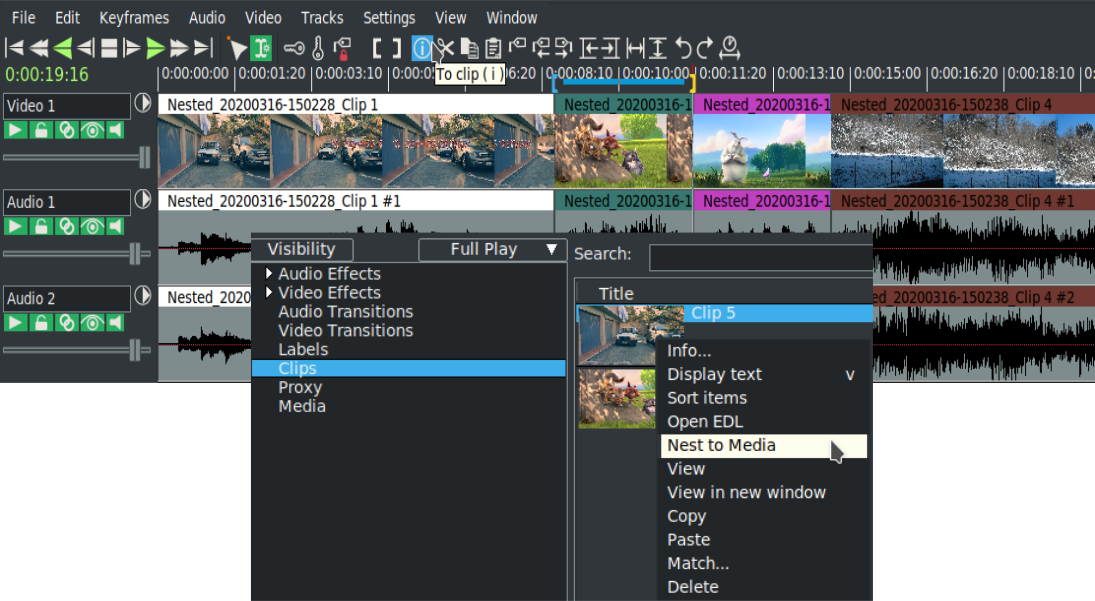
\includegraphics[width=1.0\linewidth]{nesting.png}
	\caption{Nested clips in Timeline and Resources window}
	\label{fig:nesting}
\end{figure}

\paragraph{Notes:} creating nested clips is a complicated internal process for \CGG{}, especially for managing audio tracks. Therefore you need to make sure you have your project set up as you expect before you start nesting with the \texttt{Nest to Media} command.  Below are several things to remember.

\begin{itemize}
	\item The creation of the nested clip is based on the settings in \texttt{Settings $\rightarrow$ Format}. Be sure that the number of audio tracks and channels is the same as we want to have in the nested clip. In addition, it is better to make each audio track independent from the others (which could be linked in more than one channel) using the option: \texttt{Audio $\rightarrow$ Map 1:1}
	\item You can do any editing on the nested clip once it is loaded to the timeline. For example we can start an OpenEDL session to make the changes. Once out of the OpenEDL session it may be that the changes made are not visible in the original nested clip. You can fix this by doing RMB on the nested clip in the \textit{Resources/Media} window and choosing \texttt{Rebuild index}. This process may take some time depending on the size of
the media; because of the additional time required to do this, it is not done automatically in order to allow the user to make the decision as to when they are done editing enough and need to see the exact results
in order to save time.
	\item Because of the way the timeline thumbnails are displayed, after editing using OpenEDL of a
nested clip, the thumbnails of the video track may be redrawn and may look different and out of sync with the
way they did originally with respect to the audio waveforms. This is simply a result of the redrawing of the
video track which is independent from the redrawing of the audio tracks. The playback is still synchronized.
\end{itemize}

\paragraph{Usage Examples of Nested Clips}

\begin{description}
	\item[Example 1:] You want to make a flashback/rewind at the end
	of your video that represents a quick summary of the entire video in
	black and white. On he timeline, you have 60 seconds of edits with
	clips, cuts, zoom in, zoom out and any other edits. Now you want to
	get this 60 seconds \textit{compressed} to 10 seconds, play in
	reverse, and in black and white at the end of your video.  You would
	copy the 60 seconds in a clip, nest the clip in the Clip folder of
	the Resources window and drag it to the timeline. You will see only
	a clean clip without all of the edits that were used to create it
	because nesting display a clip without having to actually use the
	Render menu.  Now you can add a Reverse effect, Color3way plugin for
	black and white, and use the Speed auto to get the 60 seconds down
	to only 10 seconds.
	\item[Example 2:] You are working on a complex project with a
	team in a separate location. You create some sub projects, i.e.\
	sequences, that you or the team will use in the Master project to
	merge the sequences in the right order and to make the final color
	correction steps.
\end{description}

In each of the examples you can see the benefit of nesting to create
clean looking timelines because of the automatic rendering
capability of nesting.

\section{Multi-Camera / Mixer}%
\label{sec:multicamera_mixer}

Use the Mixer Viewer to see multiple media playing simultaneously in re-sizable mini-viewers.  This can be used in various ways and is useful to edit videos shot by multiple cameras from different viewpoints that were simultaneously recorded in order to create a single good video.  Everything will have to be initially synced so you can decide which one of the camera angles is best suited at any time. 

The number of cameras/mixers you can have is generally limited to the available resources on your computer.  Currently, the number of File Descriptors available in the OS limits cameras to about 50.  If you have many \textit{mixer viewers} you will probably want to use proxy mode whenever possible.  Also, in the \texttt{Settings $\rightarrow$ Playback A} tab \textit{Video Out} section, uncheck \textit{play every frame} and choosing a Video Driver of \textit{X11} with \textit{use direct X11 render if possible} checked, will provide better performance.

Figure~\ref{fig:multicam01} shows 9 media sources in the left corner, the composed video in the right corner, the timeline with the top video track with pieces of the 9 overwrites, and the choice in Resources of Mixed.

\begin{figure}[htpb]
	\centering
	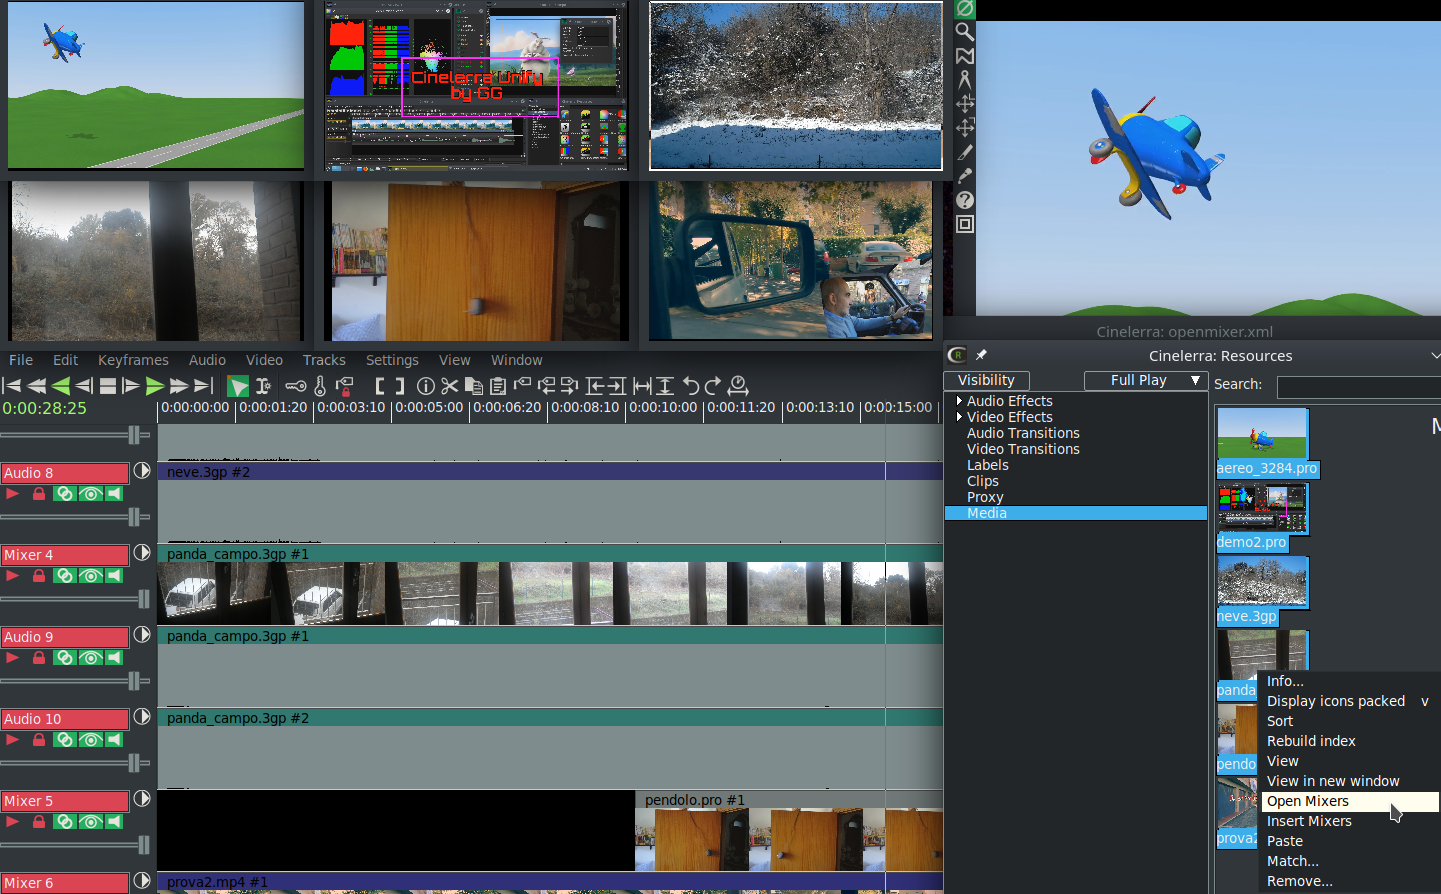
\includegraphics[width=1.0\linewidth]{multicam01.png}
	\caption{Using Mixer capability in Cin for multiple cameras}
	\label{fig:multicam01}
\end{figure}

\subsubsection*{Easiest Method to Getting Started}%
\label{ssub:easiest_method_started}

\begin{enumerate}
	\item This method assumes all of your media or cameras are aligned the way you want them already.
	\item From the \textit{File} pulldown, create a \textit{New project} with the desired format for Audio and Video output (or you can just use the default).
	\item \texttt{File $\rightarrow$ Load} the media files you want to work with using \textit{Create new resources only}.
	\item In the Resources window, with  the Media folder, highlight the list of media you want to \textit{Mix}. This is done using a ctrl or shift mouse button press as you would in a standard listbox selection.
	\item Right click the mouse on the media selection and choose \textit{open mixers}. This opens multiple mixer viewer windows, one for each media item that was highlighted.  You can
	do them 1 at a time instead.  This also adds the source media tracks to the main window.
	\item Now use the timeline to play and you will see all viewers/cameras playing.  Stop when you get to the
	end of the \textit{good} camera playback.
	\item Simply double click the \textit{good} mixer viewer and from where you first started playing to the playback insertion pointer is the source section, which will be pasted in the destination video/audio tracks at the top of the new project.
	\item Repeat steps 6-7.  Start playing again, stop when you want, double click the desired mini-viewer!
\end{enumerate}

\subsubsection*{Some Hints and Caveats}%
\label{ssub:hints_caveats}

\begin{itemize}
	\item You can easily overwrite a section of the new track by \textit{selecting} a section on the timeline, then double click on one of the mini-viewers to overwrite/replace that section.
	\item If you edit the output tracks, it only edits output tracks, and the input tracks may no longer be lined up.
	\item You can add a silent section by selecting past a section and start overwriting that section from then on.
	\item If you use the cursor hairline to create the selection endpoint, it must be past the end of the destination.
	\item The compositor shows composed media.  This is the media that will be rendered.
	\item The program always uses overwrite as the paste operation.
	\item Use the timeline edit handles to move the start and end points of that section.
	\item Only middle mouse drag handle operations should be used normally.
	\item Other drags will displace the media source/destination timeline correspondence.
	\item To re-tile the mixer windows after you have resized and moved them around, you can use the Window
	pulldown of \textit{Tile mixers} or the shortcut of Alt-t.
\end{itemize}

\subsubsection*{But, I want to use only the first set of audio tracks\dots}%
\label{ssub:but_use_only_first_audio}

There are many cases where you may want to compose using media from several different tracks while using the the same audio tracks as associated from a specific viewer.  Since mixer source tracks can be updated any time by using a mixer toggle, this makes it possible to do this.  

Procedure to update the mixer audio source track list:

\begin{enumerate}
	\item Single click to highlight the mixer window you want to re-associate to the audio track.
	\item In that audio track’s patchbay click the expand toggle, the arrow on the right side.
	\item In the expanded pane that appears, there is another arrow on the left side.  This icon has the tooltip \textit{Mixer}.  Click this and because in step \#1 you highlighted the mixer window, it will now be toggled on.  Once you click the mixer icon it will then point up.
	\item Now, disassociate any audio that is unwanted by expanding its patchbay and toggling off the mixer.
\end{enumerate}

\subsubsection*{Expert Usage}%
\label{ssub:expert_usage}

When you double click a mixer viewer window, it operates an \textit{overwrite} paste operation.  This moves \textit{src} (source) track edits to \textit{dst} (destination) track edits over the same selected timeline region.

\begin{itemize}[noitemsep]
	\item \textit{Src tracks} should be not playable and not armed in the main window patchbay gui.
	\item \textit{Dst tracks} should be playable and armed in the main window patchbay gui.
\end{itemize}

Each mixer viewer maintains a list of the tracks which will be used as src. This list is made visible selecting the window with the left mouse button.  When the mixer viewer is selected, a highlight is drawn around the media image.  All track patchbay \textit{mixer} toggles are updated to reflect the src tracks included in the selected viewer src track list. The track patchbay toggles can be used to manage the list.

\begin{itemize}[noitemsep]
	\item \textit{Turning on} a toggle (pointing up) includes the track in the src track list.
	\item \textit{Turning off} a toggle (pointing right) removes the track from the src track list.
\end{itemize}

New Mixer viewers can be created using the main menu \texttt{Window $\rightarrow$ Mixer Viewer}, or with a shortcut of \texttt{Shift-M}.  When a new viewer is created, the currently enabled patchbay \textit{mixer} toggles are used to create the viewer source track list.  The toggles are cleared after the window is created.  This is to improve the work flow.  Use the following list of steps to create individual mixer viewers.

To create a list of mixer viewers:

\begin{enumerate}
	\item Setup the session \texttt{settings $\rightarrow$ format}, width, height, frame rate, color model, aspect ratio.
	\item Create dst tracks using the a/v track pulldowns (or use shortcuts "t" / "T"),  armed and playable.
	\item Append src tracks using \texttt{file $\rightarrow$ open $\rightarrow$ append tracks}, or the resource window using pasting.
	\item Using the track patchbay, disarm editing and disable playback of the audio/video src tracks.
	\item Using the track patchbay, mark the new tracks as \textit{mixer} source to be added to the viewer.
	\item Create a mixer viewer using the main menu pulldown, or the shift "M” shortcut.
	\item Repeat steps $3-6$ for each mixer viewer needed for the session editing.
\end{enumerate}

When you single click a mixer window, it becomes selected and highlighted and all of the patchbay mixer toggles are updated to reflect the state of the viewer’s src tracks.  Tracks that will be src are shown as enabled.  If you change a toggle, the src tracks for the selected window will be modified.  This means you can associate or dis-associate any media track to any mixer window.

When you double click a mixer window, an overwrite paste is invoked.  The mixer viewer’s src tracks are overwritten to the dst tracks.  The timeline region for both the source and destination are the same for the overwrite paste function.  The selection region is used if it is active.  If the selection is empty, that is it is a hairline, the selection region is from the end of the destination playable edits to the selection cursor hairline.  The hairline must be past the end of the playable edits on the destination tracks.

The mixer viewer configuration is saved with the session data.  When a saved session is loaded in \textit{replace project} or \textit{replace project and concatenate tracks}, the mixer viewer will be reopened.

\subsubsection*{Using Proxy with \textit{Open Mixers}}%
\label{ssub:using_proxy_open_mixers}

The best way to use proxy with your multiple cameras is to follow the steps below:

\begin{enumerate}
	\item Load media with insertion strategy of \textit{create resources only}.
	\item Highlight the media in the Resources window and right click on this to choose \textit{open mixers}.
	\item Use the \texttt{Settings $\rightarrow$ Proxy settings}\dots to bring up the proxy menu.
	\item Choose the size and other options you want and click the checkmark OK. If you choose the option \textit{Beep when done} you will hear a short beep if all media is already proxied or a longer beep when all proxies have been created.
	\item When your editing is complete, use \textit{Settings} pulldown and proxy to \textit{original size}.
\end{enumerate}
Instead of Open Mixers, you can Insert Mixers with new tracks at the timeline insertion point.

\begin{figure}[htpb]
	\centering
	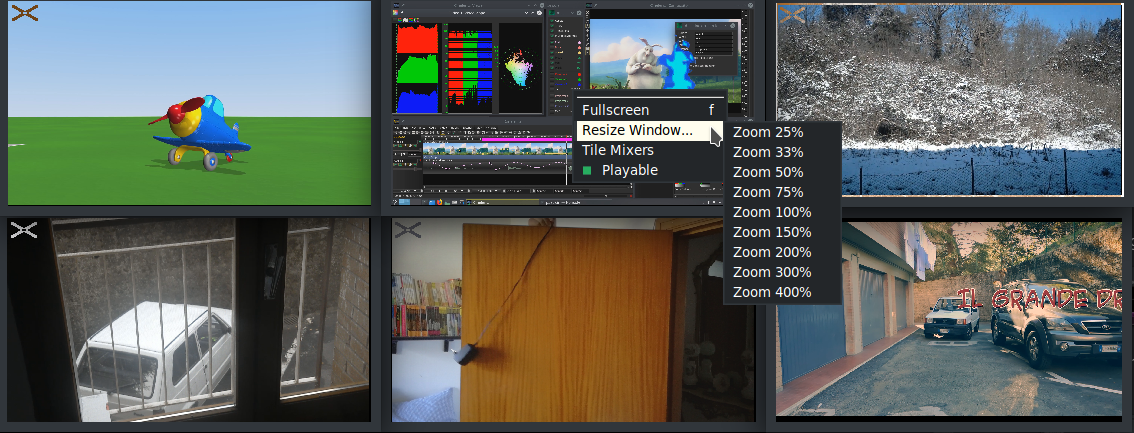
\includegraphics[width=1.0\linewidth]{mixer-playable.png}
	\caption{A Mixer window showing available options with the white X designating no playing}
	\label{fig:mixer-playable}
\end{figure}

\subsubsection*{Options available in the \textit{Mixer Windows}}%
\label{ssub:options_available_with_mixers}

There are several options you will see in each Mixer window that help with using them. These
are shown in figure~\ref{fig:mixer-playable}. To use these, RMB in the desired mixer window,
and choose one of the options as described here.

\begin{enumerate}
	\item Fullscreen / Windowed - will bring up a fullscreen display of that window or revert to the original size.
	\item Resize Window - allows for resizing the window to a choice of different sizes.
	\item Tile Mixers - makes it easy to get all of the mixers nicely tiled to a standard size.
	This is also available in the Window pulldown.
	\item Playable - enabled by default so that you will see a checkmark next to it in the 
	popup.  The benefit of making a mixer window not playable is to save cpu time. When a specific
	mixer window is unchecked, so not Playable, a white cross appears in the upper left hand corner
	of the mixer.  To switch back to playing again, RMB and choose Playable and this will turn
	playing back on. The program automatically updates the mixer image when the timeline cursor
	stops or when it is moved to a different spot even when play is disabled. You can see the
	white cross designating not playable in figure~\ref{fig:mixer-playable}. Statistics that show
	the savings are as follows on a 16 cpu laptop:
	\begin{verbatim}
	5 Mixers all playing -- cpu usage = 1275
	1 only playing       -- cpu usage =  405
	2 only playing       -- cpu usage =  800
	\end{verbatim}
\end{enumerate}


\subsection{Recover Mixer Windows}%
\label{sub:recover_mixer_windows}

It is a hazard that you might accidentally \textit{undo} (\texttt{z}) too far and lose your mixer windows.  Here are the steps to recover.  It is recommended that you make a backup of your project before performing the recovery steps just in case there are other problems.

In the patchbay box to the left of the main timeline, there is a right pointing arrow on the right side.  This is called the \textit{Expander} (figure~\ref{fig:mixer-patchbay01}).  When you click on each expander, another line appears below that expander arrow and the timeline track height is slightly increased.  If you Shift-click on a single expander, the patchbay will expand for all of the tracks.

\begin{figure}[htpb]
	\centering
	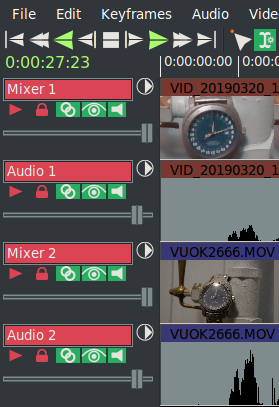
\includegraphics[width=0.35\linewidth]{mixer-patchbay01.png}
	\caption{Mixer  patchbay}
	\label{fig:mixer-patchbay01}
\end{figure}

\begin{enumerate}
	\item Expand all of the patchbay lines, either one by one, or Shift-click on one to do them all. This is so you can see the \textit{mixer} right pointing arrow on the second expanded line.    
	\item Use the Window pulldown and choose \textit{Mixer Viewer} to bring up a new mixer window.  Now you will be making an association between the mixer viewer and the track’s video.
	\item Click on the new mixer window to make sure it is highlighted with a white border. This designates it as the \textit{in use} mixer viewer.
	\item Set your play to the beginning of the video using the \textit{Home} key or \textit{Home} transport button.
	\item In the patchbay for a video track click on the \textit{mixer} arrow on the expanded $2^{nd}$ line which is a right facing arrow.  Now the arrow will point up.  If there are audio tracks with that video, click on each of its audio tracks \textit{mixer} arrow until they point up also.
	\item Next move your insertion pointer on the timeline where there is video.  Some of the time this just helps so that the new mixer viewer window gets redrawn and you can see that the images appear; but the image may not appear until the program does a redraw later.  Now the mixer viewer should be
	correctly associated.  Note if you have large video, give it some time to update.  You may have to click on the mixer viewer window if the image does not show.  You can always start over with that mixer if you encountered any problems.
	\item Click the arrows that are pointing up in that video and its audio so they go back to pointing right. That mixer viewer is complete so you need to do this to make sure the \textit{mixer} arrows are off.
\end{enumerate}

Repeat steps 2 through 7 for each of the mixer viewers you need going down the patchbay starting on step 2 first with Mixer 1, then 2 to 7 steps for Mixer 2, then again run 2 to 7 for Mixer 3 and so on.

Sometimes the association does not stick initially.  If not, highlight the mixer viewer with the problem, change the mixer arrows to point up, and reassociate.

\section{Audio/Video sync via Waveforms/Timecodes}%
\label{sec:audio_video_sync}

\subsection{Audio/Video sync via Waveform}%
\label{sub:audio_video_sync_waveform}

Multi-camera footage of a single event can have various shots starting and ending at different times. So when the footage start times are different, you can use the mixer audio to synchronize the clips on the timeline. The program algorithm attempts to find and align automatically the waveforms of the media.

Synchronizing multiple camera videos based on audio tracks can be done with \CGG{} easily enough with the \texttt{Window $\rightarrow$ Mixers$\dots$ $\rightarrow$  Align mixers} option.  Align mixers brings up a window displaying your mixers, the currently selected Master Track, and a list of all of the Audio Tracks (figure~\ref{fig:mixer-align01}).  There is a limit of 32 audio tracks per each mixer (that should be enough!)

\begin{figure}[htpb]
	\centering
	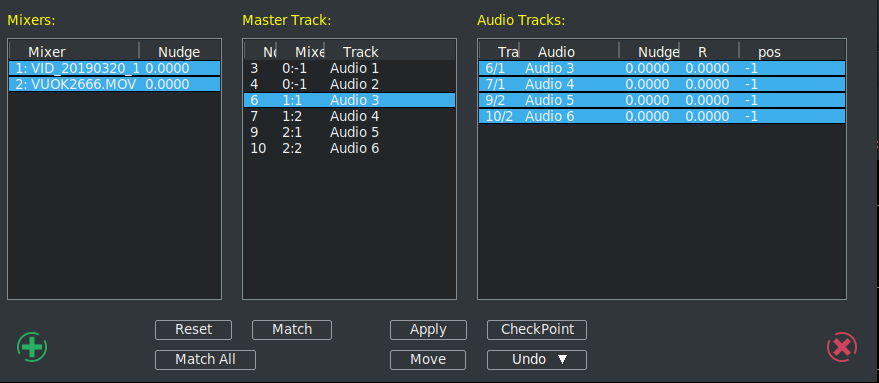
\includegraphics[width=0.9\linewidth]{mixer-align01.png}
	\caption{Align Mixers window}
	\label{fig:mixer-align01}
\end{figure}

Two different methods of aligning the audio for mixers are available. They are most easily referred to by the button that is pressed -- \textit{Match} and \textit{Match All}. There are also 2 methods of activating the alignment -- \textit{Apply} and \textit{Move}.  

\textit{Match} consists usually of the next set of steps to take advantage of this feature:

\begin{enumerate}
	\item Load your camera media with insertion strategy of \textit{resources only}
	\item Highlight in the Resources window, all of the media you want to mix.
	\item Right mouse button on one of the media and click on Open Mixers; all mixer windows come up.
	\item To arm the created mixer tracks and related audio tracks. They are automatically placed on the timeline disarmed. This is right for multi-cam but not for audio sync.
	\item Provide a small target audio pattern on the Master Track for syncing by marking with the In/Out points ([ and ]). NOTE: When choosing between the audio tracks to align the one that will have to work as Master, we must rigorously use the one with the right-most synchronization peak. This is because the Master track will be started at the beginning of the timeline. If during alignment the other tracks should move further to the left than the Master, they will be truncated at 00:00:00:000, finding no more space available, and will be shortened with loss of footage for the next multi-cam
	\item Make a selection on the timeline in which to look for the pattern. Left mouse click, then drag select and highlight a search time domain. 
	\item Use the \texttt{Window $\rightarrow$ Mixers$\dots$ $\rightarrow$  Align mixers} to bring up its dialog window.
	\item Highlight in the first listbox, the Mixer number you want to align. Click on \textit{Match}. This will take a few seconds so watch the rendering time percentage on the lower right hand side zoom panel. The buttons will be ghosted out until finished. Now note the changed values in the Audio Tracks listbox.
	\item If you are satisfied with the calculated Nudge values -- that is they are very close to $1.0$ -- in the Audio Tracks listbox and the audio track selected as the Master Track in the Master Track listbox, hit the \textit{Apply} button.
	\item If you plan on performing more alignment tasks, click on Checkpoint so you can go back to a previous step in case you make a mistake.
	\item Last, click on the OK green checkmark or to cancel click on the red X.  Or just close the gui.
	\item To disarm the mixer tracks and related audio tracks for the next multi-cam operations.
\end{enumerate}

\paragraph{Reset} is used to start over with the current session data, not an undo.  This means you can use the match repeatedly to refine alignments.  All of the Audio Tracks listbox values will be reset.

\paragraph{Checkpoint} provides a method to create checkpoints that save the current state.  This is especially helpful while learning or doing more complicated operations where you might make a mistake or do not like the results and need to get back to a previous state.

\paragraph{Undo} is used to put the media back to a previous state on the timeline.  If you choose \textit{start over} the session will reload with the original, before any changes were applied.  You can also go back to any of your previous checkpoints that you created earlier which are listed there, such as \textit{chkpt 1}.

\paragraph{Match All}is used when you have several mixers, instead of only picking 1 to match, it picks the best match for EACH of the mixer tracks based on a single master track. So when you hit Apply, each track might move differently. You do not set In/Out points but you have to make a selection within which to match.

\paragraph{Apply} button will apply the nudges that were generated during the Match or Match All execution (figure~\ref{fig:mixer-align02}).

\begin{figure}[htpb]
	\centering
	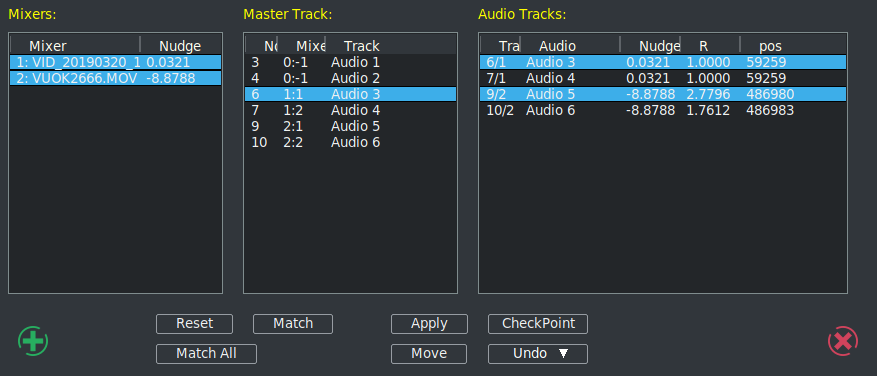
\includegraphics[width=0.9\linewidth]{mixer-align02.png}
	\caption{Aligned mixer window after "Match". Note the Nudge amounts above.}
	\label{fig:mixer-align02}
\end{figure}

\paragraph{Move} is very handy when you are using mixers, if you have an edit somewhere that you need to fix specifically without moving any of the other track pieces. In this case you have to select a section (like you do a group, but do not make a group), generate a match, and then you can just \textit{Move} that set only -- everything else stays where it is at its current location (figure~\ref{fig:mixer-align03}).

\begin{figure}[htpb]
	\centering
	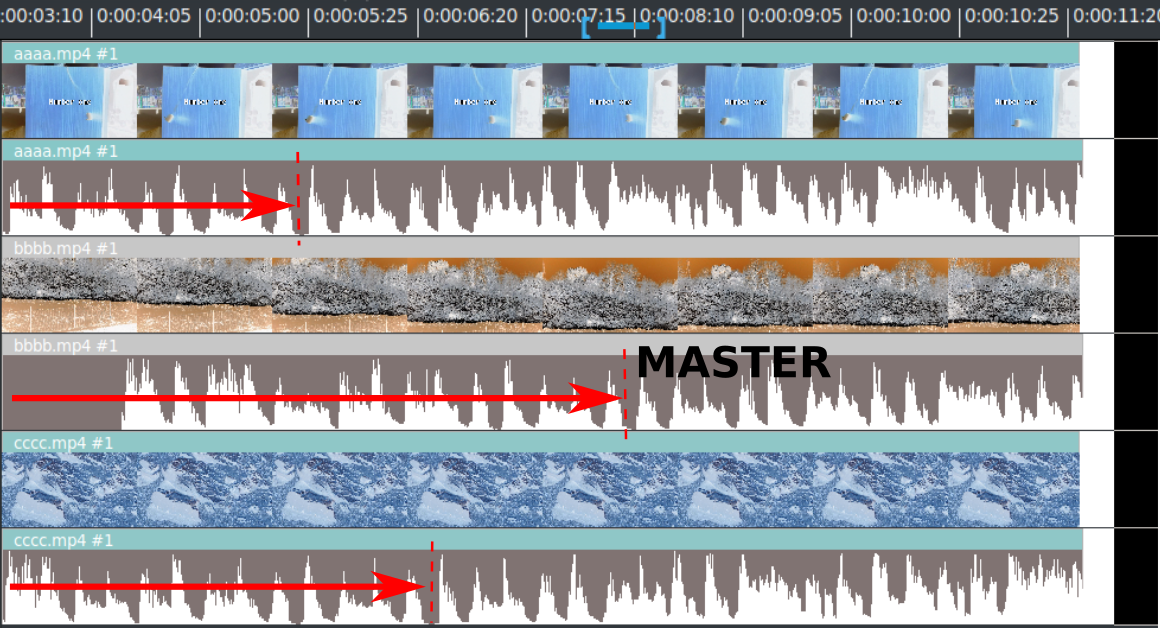
\includegraphics[width=1.0\linewidth]{mixer-align03.png}
	\caption{Match setup for aligning by audio.  Note that [ ] are set over a sample waveform highlighted selection that includes that.}
	\label{fig:mixer-align03}
\end{figure}

More detailed information follows about how this all works and the information in the dialog window.  It is important to know that the result of the calculation is \textit{best match} but you can still override the selections if you decide there is a better one.  The dialog window is split into 3 sections:

\begin{enumerate}
	\item \textit{Mixers} lists the mixers that are active by highlighting them all initially. You can decide that you do
	not want 1 or more mixers to be used in the correlation calculation by un-highlighting the one(s) that should not be used. In some cases you have to have at least 2 in order to align audio.
	\item \textit{Master Track} lists each of the audio tracks currently loaded for all of the mixers. You can decide to highlight a different audio track to be used as the master for correlation, but only 1 can be used. Remember to use the track with the right-most synchronization peak as the Master.
	\item \textit{Audio Tracks} lists each of the mixer audio tracks.  Again, you can highlight a different set of which
	mixer audio tracks that you want to use for the waveform correlation.  Any audio tracks that are not
	highlighted, that is \textit{turned off}, will not be considered in the correlation calculation.
\end{enumerate}

The corresponding input position is determined by track input correlation.

The letter "R" in the Audio Tracks listbox represents the correlation value.  $R=1.0$ designates that if both the pattern and the matching section were in the highlighted area, they are completely correlated -- this is a good self-test to check.
$Nudge=0.0$ means just that.

The header \textit{pos} stands for the timeline position. When the \textit{Apply} button is pressed, only the Mixers listbox is relevant at that time.

The Mixer with the master track generally does not move, everything else will be lined up (figure~\ref{fig:mixer-align04}).

\begin{figure}[htpb]
	\centering
	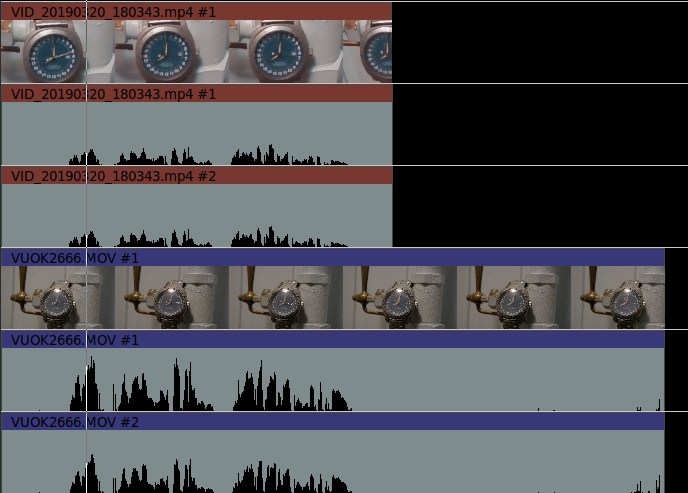
\includegraphics[width=1.0\linewidth]{mixer-align04.png}
	\caption{An audio Match is complete. Note the waveform is aligned.}
	\label{fig:mixer-align04}
\end{figure}

\textit{Match All} option basically consists of the following steps:

\begin{enumerate}
	\item Highlight the Mixer to use in the Mixer listbox.
	\item Highlight the Master Track you want to use in the Master Track listbox.
	\item On the timeline, mark your selection on the Master Track.
	\item Click on the \textit{Match All} button.
	\item Note the nudge values to see if they make sense, and if so, press \textit{Apply}.
\end{enumerate}

\textit{Match} option basic steps (just for comparison with Match All):

\begin{enumerate}
	\item Set the In/Out points [ ] of the target.
	\item On the timeline, mark your selection.
	\item Click on the \texttt{Match} button.
	\item Note the nudge values to see if they make sense, then press \textit{Apply} (or \textit{Move} when doing a group).
\end{enumerate}

\subsection{Align Timecodes}%
\label{sub:align_timecodes}

Align Timecodes is especially useful in the case where you create video with multiple cameras capable of recording a timecode in the metadata of each file.  Let’s say we have recorded three videos at the same time at a concert with each camera set up at unique positions and at different angles.   All of the cameras start recording at various times but were synchronized with the same master clock (\textit{Timecode Sync Generator} or \textit{Jam Sync timecode}) so that the recordings are timestamped with that synchronized time.  For example, the 3 cameras have embedded metadata as follows: \quad \textbf{camera 1} = 00:00:00:01 \quad \textbf{camera 2} = 00:00:10:07 \quad \textbf{camera 3} = 00:00:17:22

\begin{figure}[ht]
	\centering
	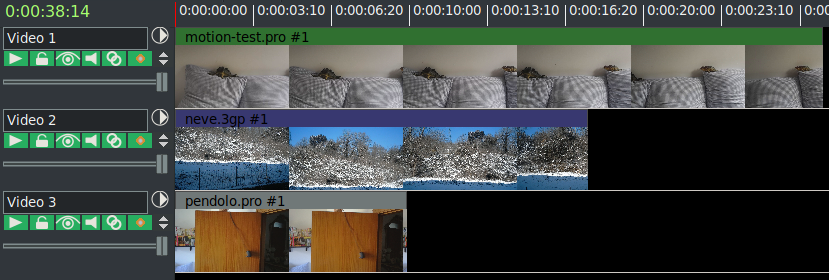
\includegraphics[width=1.0\linewidth]{timecode-01.png}
	\caption{Before sync}
	\label{fig:timecode-01}
\end{figure}

Timecode synchronization is performed by the program when you choose the option \textit{Align Timecodes} and works in 2 steps. The first automatic step is to locate the earliest timecode and the second step is to align the edits on the armed tracks using that time on the timeline. 

When you load in the three files to different tracks, they'll be placed on a timeline that starts from $00:00:00:00$ as usual. But, by middle mouse clicking (MMB) on any of the video tracks, you can view the timecode embedded at that point in that file.

To make it easy to align the videos onto the timeline manually, set the \textit{origin point}, that is the leftmost time index, of the timebar to the timecode of the earliest video.  For the 3 aforementioned cameras this would be camera 1 with a timeecode of $00:00:00:01$.  By using the \textit{clapboard} button on the main timeline, you can set $00:00:00:01$ as the start timecode. Then positioning the camera 1 video at the start of the timeline will line its frames up with the times on the timebar.

\begin{figure}[ht]
	\centering
	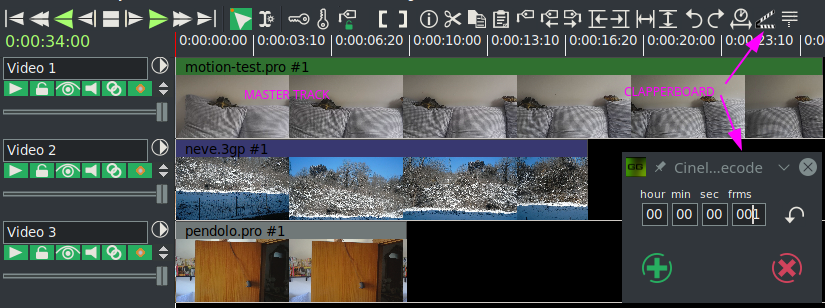
\includegraphics[width=1.0\linewidth]{timecode-02.png}
	\caption{Clapperboard button}
	\label{fig:timecode-02}
\end{figure}

Similarly, using the middle mouse button to view the other 2 camera’s timecodes, you can position them  so their timecodes line up and now all three tracks will be in sync.  You can do this manually or simply do it automatically with the option under: \texttt{Tracks  $\rightarrow$  Align Timecodes}. See figure~\ref{fig:timecode-03}

\begin{figure}[ht]
	\centering
	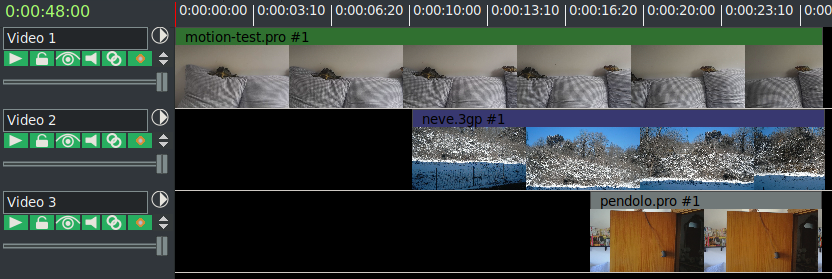
\includegraphics[width=1.0\linewidth]{timecode-03.png}
	\caption{After sync}
	\label{fig:timecode-03}
\end{figure}

Timecode synchronization in \CGG{} is based on the inclusion of an actual \textit{timecode} saved in
the media as can be seen using the \texttt{ffprobe} or \texttt{mediainfo} command line. Examples are shown here:

\begin{lstlisting}[style=sh]
# ffprobe tut1.mov
Metadata:
handler_name:	VideoHandler
timecode:		00:00:20:01

# mediainfo mtb.mp4
Time code of first frame:	11:05:49:41
Time code, striped:		Yes
Title:				GoPro AVC
\end{lstlisting}

Many newer cameras and media in a MOV container have valid timecodes often with SMPTE
compliant start Timecode in Quicktime format, whereas others do not. Most low end cameras do not.
When no timecode is present, various clock time values may be used to synchronize instead.

There are various types of timecodes and they are written in metadata in various ways. Because it is not clear which timecode in the file is the one to use or there is none, the precedence as described next is followed. The contexts, packets, streams, and data refer to the corresponding ffmpeg data or metadata objects:

\begin{enumerate}
	\item if the format context has a timecode use: \texttt{fmt\_ctx $\rightarrow$ timecode - 0}
	\item if the layer/channel has a timecode use: \texttt{st $\rightarrow$ timecode - (start\_time -nudge)}
	\item find the first program stream with video stream, and if the video stream has a timecode use:
	\texttt{st $\rightarrow$ timecode - (start\_time-nudge)}
	\item find timecode in any stream use: \texttt{st $\rightarrow$ timecode}
	\item read 100 packets, save \texttt{ofs=pkt.pts*st $\rightarrow$ time\_base - st $\rightarrow$ nudge}:
	\begin{itemize}
		\item decode frame for video stream of the first program
		\item if \texttt{frame $\rightarrow$ timecode} has a timecode use:\texttt{ frame $\rightarrow$ timecode - ofs}
		\item if side\_data has gop (group of pictures) timecode use: \texttt{gop $\rightarrow$ timecode - ofs}
		\item if side\_data has smpte timecode use: \texttt{smpte $\rightarrow$ timecode - ofs}
	\end{itemize}
	\item if the \texttt{filename/url} scans \texttt{*date\_time.ext} use: \texttt{date\_time} (yr, month, day, hr, min, sec, nanosecond)
	\item if stat (display file status) works on the \texttt{filename/url} use: \texttt{mtime} (modification time)
	\item finally, if none of the above are usable, then return \texttt{failure}
\end{enumerate}

Operation of Align Timecodes includes the following options to help in your setup and review (figure~\ref{fig:timecode-04}):

\begin{figure}[ht]
	\centering
	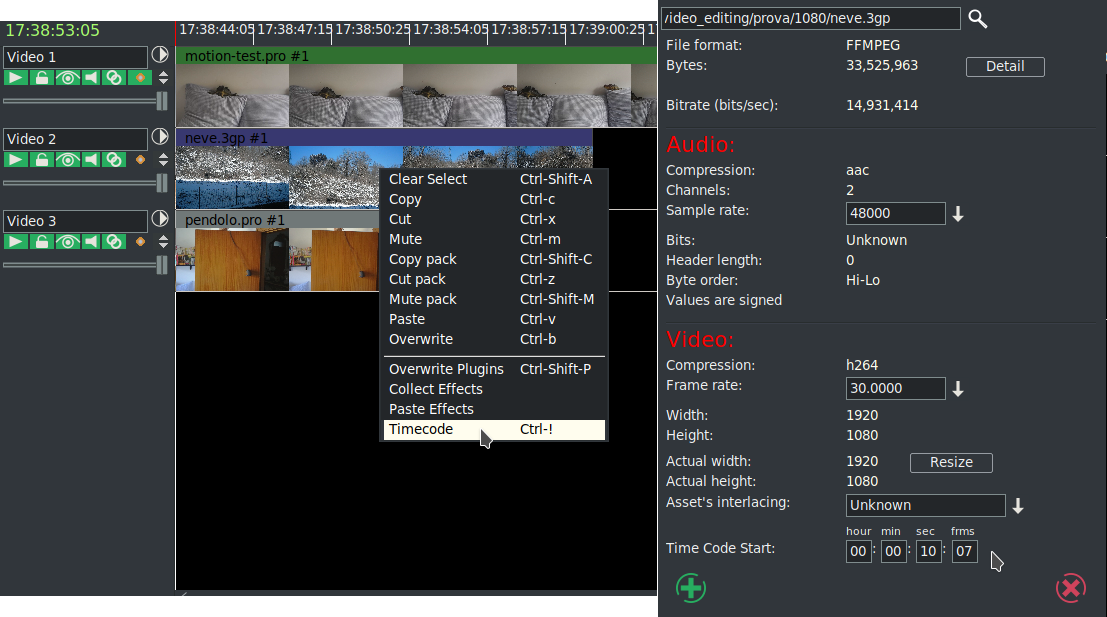
\includegraphics[width=1.0\linewidth]{timecode-04.png}
	\caption{Timecode via MMB on track and via Resources windows/Info}
	\label{fig:timecode-04}
\end{figure}

\begin{itemize}
	\item \textit{Align Timecodes} under the \textit{Tracks} pulldown
	\item \textit{Clapperboard} icon on the main timeline to set a timecode.
	\item Timecode option added to timebar choices (in timecode $hh:mm:ss:ff$) with use of the session frame
	rate as a time standard.
	\item Time Code Start in the Resources window on the bottom of \textit{Info} for the media if the timecode for that
	asset has been scanned and is known. You can scan the asset’s Timecode by using the middle mouse
	button on its track which then displays the timecode for that on the timebar.
\end{itemize}

\paragraph*{Notes}

\begin{itemize}
	\item \textit{Align Timecodes} is a good first step to quickly sync media up either perfectly or roughly.
	\item Currently this is not known to function for syncing audio recorded on a separate audio device,
	because no test material was provided to ensure that this works.
	\item Disarmed tracks will not be affected by using \textit{Align Timecodes}.
	\item No edits or sections will get cut off on the left or elsewhere, unless the moved edits overlap.
	\item You can add a timecode to video using an \texttt{ffmpeg} command if you want to align a particular video
	which has no timecode to ones that do. For example:
\end{itemize}

\begin{lstlisting}[style=sh]
ffmpeg -i originalfile.mp4 -metadata timecode="14:36:08:29" -c copy newfile.mp4

# where "-i" is followed by the input filename
# where "-metadata timecode" is followed by the timecode key
# where "-c copy" just copies the video/audio to the following output filename
\end{lstlisting}

